\section{Experiments}
\label{sec:exp}

All rules use $16{\times}16$ patches on 8-bit grey frames. Unless stated, the range rule runs at $\Delta = 32$ and the multi-scale rule at $\Delta_0 = 80$ with box half-widths $r \in \{0,1,2,3\}$ and $\Delta_r = \Delta_0 (2r+1)^{-1/2}$, the operating points of \citet{nair2026certifiedskip}. Soundness is always audited the same way: on a random sample of dropped patches, the persistence diagrams of $F$ and of the reference the rule actually constructed are computed exactly, and Theorem~\ref{thm:warp} is checked against them. Every number below is produced by a script in the repository from a stored output file (Appendix~\ref{app:repro}).

\subsection{Moving cameras: DAVIS 2017}
\label{sec:davis}

DAVIS~2017 \citep{ponttuset2017davis} has 90 train and validation clips at 480p, shot with moving and mostly handheld cameras, with a pixel mask of the moving objects in every frame. We run the first 40 frames of every clip. The masks split the patches into \emph{object} patches (overlapping an annotated object) and \emph{background}, so that a high drop rate can be checked to come from the background rather than from losing the objects. Five rules are compared: the fixed-camera range rule and quotient + multi-scale, which see a moving camera as change everywhere, and three warp rules: the per-frame homography with the range certificate, the same with per-patch refinement ($|\delta|_\infty \le 1$~px), and the same with the multi-scale certificate (Table~\ref{tab:davis}, Figure~\ref{fig:davis}).

\begin{table}[t]
\centering\scriptsize
\setlength{\tabcolsep}{4pt}
\begin{tabular}{lrrrrrrr}
\toprule
rule & drop & drop, object & drop, backgr. & revealed & cuts/clip & $\iota$ median & ms/frame \\
\midrule
fixed range & 0.212 & 0.047 & 0.208 & 0.000 & 0.00 & 0 & 2 \\
fixed quotient+MS & 0.435 & 0.182 & 0.469 & 0.000 & 0.00 & 0 & 145 \\
warp range & 0.436 & 0.067 & 0.485 & 0.038 & 1.67 & 31 & 1013 \\
warp+refine range & 0.494 & 0.091 & 0.555 & 0.036 & 1.20 & 33 & 1398 \\
warp+refine MS & 0.728 & 0.233 & 0.807 & 0.037 & 0.74 & 44 & 1324 \\
\bottomrule
\end{tabular}

\caption{DAVIS~2017, all 90 clips, first 40 frames each; medians over clips. ``Revealed'' is the share of patches kept because their area was not yet in the canvas. ``Cuts/clip'' counts frames on which registration failed and the canvas was reset. $\iota$ is the median interpolation term of Proposition~\ref{prop:iota} in grey levels. Times are for the Python prototype with nine clips processed in parallel on one laptop, so they overstate single-stream cost.}
\label{tab:davis}
\end{table}

\begin{figure}[t]
\centering
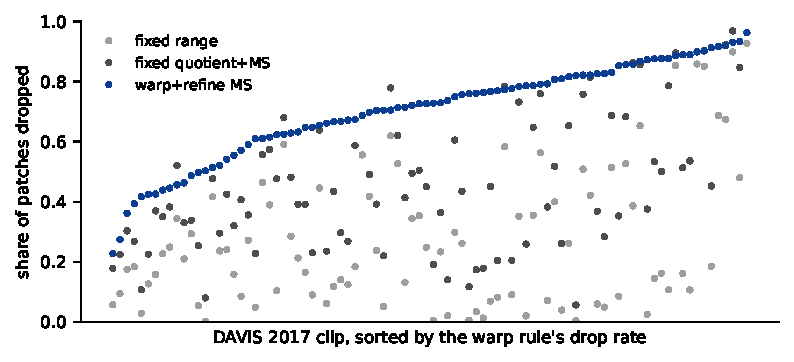
\includegraphics[width=0.66\linewidth]{figures/davis_drop}\hfill
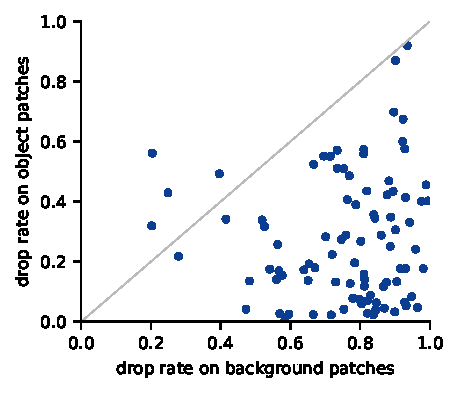
\includegraphics[width=0.33\linewidth]{figures/davis_object_vs_background}
\caption{Left: share of patches dropped on each DAVIS clip, sorted by the full warp rule. Right: for the full warp rule, drop rate on object patches against background patches, one point per clip; points below the diagonal drop less on the objects than on the background.}
\label{fig:davis}
\end{figure}

The full warp rule drops a median of 72.8\% of patches, against 43.5\% for the fixed-camera quotient + multi-scale rule and 21.2\% for the fixed range rule. It drops more than the fixed rule on 81 of the 90 clips, by a median of 20 points; across clips its drop rate runs from 46\% at the 10th percentile to 89\% at the 90th. Registration alone (warp range, 43.6\%) only matches the fixed quotient rule; the per-patch refinement adds six points and the multi-scale certificate another 23, which is the same order of gains as on fixed cameras: jitter of sharp edges, now including the residual jitter left by an imperfect homography, is what the range statistic spends its budget on.

The drop comes from the background. The full rule drops 80.7\% of background patches and 23.3\% of object patches, and it drops fewer object than background patches on 86 of the 90 clips. The objects in DAVIS move independently of the camera, so they are not explained by the frame warp and are mostly kept, which is the desired behaviour; what is dropped on objects is largely their interior, which can be locally static. About 4\% of patches are kept because their area has just entered the frame and has no reference, and registration fails on 22 of the 90 clips at least once (0.74 frames per clip on average), each time costing a full frame.

Soundness was re-checked with exact persistence diagrams on 20{,}242 dropped patches across the three warp rules (6{,}830 for the full rule), against the warped reference each rule constructed. There is no violation. The worst ratio of bottleneck distance to $s/2$ is 1.000 up to rounding: Theorem~\ref{thm:warp}(b) is attained and never exceeded, as on fixed cameras.

The price is the interpolation term. Its median over clips is 44 grey levels for the full rule. Per pixel, 4\% of the pixels of dropped patches have $\iota \le 0.5$, 69\% have $\iota \le 16$ and 96\% have $\iota \le 64$. So relative to the warped reference the certificate is exact at contrast $\Delta$, but relative to the kept pixels themselves it is, on a typical pixel, a statement at contrast $\Delta + 2\iota$, and on sharp edges a weak one. Section~\ref{sec:limits} returns to this.

\subsection{A film with cuts}

Tears of Steel (CC-BY, 720p) is cut like a feature film: handheld and dolly shots, close-ups, and a cut every few seconds. We take three 60-s excerpts starting at 120, 360 and 540~s, sampled at 6~fps and scaled to $960{\times}400$ (Table~\ref{tab:film}). The full warp rule drops 75\%, 75\% and 64\% of patches, against 65\%, 65\% and 54\% for the fixed-camera quotient + multi-scale rule. It treats 54 frames as cuts across the three excerpts, real shot changes and registration failures alike, and keeps every patch on each of them, so cut-heavy footage pays for its cuts. The certificate was re-checked on 2{,}046 dropped patches with no violation.

\begin{table}[t]
\centering\small
\begin{tabular}{lrrrrr}
\toprule
rule & drop, 120s & drop, 360s & drop, 540s & cuts & $\iota$ median \\
\midrule
fixed range & 0.478 & 0.496 & 0.310 & 0 & 0 \\
fixed quotient+MS & 0.650 & 0.653 & 0.543 & 0 & 0 \\
warp range & 0.635 & 0.630 & 0.421 & 54 & 21 \\
warp+refine range & 0.677 & 0.675 & 0.481 & 54 & 22 \\
warp+refine MS & 0.752 & 0.753 & 0.640 & 54 & 25 \\
\bottomrule
\end{tabular}

\caption{Tears of Steel, three 60-s excerpts at 6~fps. ``Cuts'' counts frames on which registration failed and the canvas was reset, summed over the excerpts; the fixed-camera rules have no notion of a cut.}
\label{tab:film}
\end{table}

\subsection{Soundness of the warp certificate on synthetic scenes}
\label{sec:warpaudit}

Footage cannot test the part of the argument that Proposition~\ref{prop:iota} leaves to measurement: whether the features of the kept content survive in the warped reference. Synthetic scenes can, because the content is known. Four scene types (smooth blobs, sharp edges, fine texture, and a mixture) are re-rendered under three warp families: whole-pixel translations, sub-pixel translations and random homographies (Table~\ref{tab:warpaudit}). Over 2{,}431 dropped patches there is no violation of Theorem~\ref{thm:warp} and none of Proposition~\ref{prop:iota}, either per pixel or on the diagrams, and in every configuration $W$ has at least as many features of contrast $\ge \Delta - 2\iota$ as the re-indexed kept pixels have of contrast $\ge \Delta$, 4{,}900 features in all. This is a count, not a matching: it shows that no $\Delta$-feature is lost to interpolation in number, not that each is matched to itself. Under whole-pixel translations $\iota$ is zero on every pixel, as the proposition says. Under sub-pixel warps its median is 8--24 grey levels, and it is largest on the edge and mixed scenes, which are also the scenes where the rule keeps most: of the 225 sub-pixel edge patches it drops 156, of the 204 homography edge patches 110.

\begin{table}[t]
\centering\scriptsize
\setlength{\tabcolsep}{4pt}
\begin{tabular}{llrrrrrr}
\toprule
warp & scene & dropped & Thm.~\ref{thm:warp} viol. & Prop.~\ref{prop:iota} viol. & $\iota$ median & $\iota$ p90 & $\Delta$-features surviving \\
\midrule
integer & smooth & 237/237 & 0 & 0 & 0.0 & 0.0 & 1.00 of 443 \\
integer & edges & 240/240 & 0 & 0 & 0.0 & 0.0 & 1.00 of 478 \\
integer & texture & 243/243 & 0 & 0 & 0.0 & 0.0 & 1.00 of 513 \\
integer & mixed & 253/253 & 0 & 0 & 0.0 & 0.0 & 1.00 of 569 \\
subpixel & smooth & 225/225 & 0 & 0 & 8.2 & 16.2 & 1.00 of 408 \\
subpixel & edges & 156/225 & 0 & 0 & 12.5 & 51.6 & 1.00 of 303 \\
subpixel & texture & 225/225 & 0 & 0 & 16.2 & 27.1 & 1.00 of 455 \\
subpixel & mixed & 163/225 & 0 & 0 & 24.0 & 75.5 & 1.00 of 345 \\
homography & smooth & 226/226 & 0 & 0 & 7.9 & 15.5 & 1.00 of 433 \\
homography & edges & 110/204 & 0 & 0 & 11.1 & 33.2 & 1.00 of 204 \\
homography & texture & 218/218 & 0 & 0 & 18.2 & 29.3 & 1.00 of 463 \\
homography & mixed & 135/222 & 0 & 0 & 20.2 & 74.3 & 1.00 of 286 \\
\bottomrule
\end{tabular}

\caption{Synthetic audit of the warp certificate. ``Viol.'' counts dropped patches on which the stated bound fails, checked with exact persistence diagrams. The last column counts features of contrast $\ge \Delta$ in the re-indexed kept pixels and the share of that count matched by features of $W$ of contrast $\ge \Delta - 2\iota$.}
\label{tab:warpaudit}
\end{table}

\subsection{The causal rule against the clairvoyant optimum}
\label{sec:compexp}

For every patch of three fixed-camera clips (hall monitor, the CAVIAR lobby, VIRAT) we compute the anchored rule's keeps $m_\theta$ and, by dynamic programming with full knowledge of the sequence, the fewest keeps $\OPT_\theta$ and $\OPT_{\theta/2}$ of any sound schedule, for the range statistic at $\theta \in \{16, 32, 48\}$ and the $L^1$ mean at $\theta \in \{2, 4, 8\}$ (Table~\ref{tab:competitive}). Theorem~\ref{thm:opt}(i) and (ii) hold on every patch. Summed over a clip, the ratio $m_\theta / \OPT_\theta$ is between 1.002 and 1.183 in all 18 settings: at the \emph{same} guarantee, the causal rule keeps at most 18\% more than a schedule that knows the future. The worst single patch is 16 times the optimum (lobby, range at 32), which is the unbounded gap of Section~\ref{sec:opt} occurring in practice on a handful of patches whose content alternates around a value the rule never anchors on. The factor two of Theorem~\ref{thm:opt}(ii) is far from binding: $\OPT_{\theta/2}$ is often several times $m_\theta$, because halving the guarantee costs any schedule more than causality costs the anchored rule.

\begin{table}[t]
\centering\scriptsize
\begin{tabular}{llrrrrrr}
\toprule
clip & statistic, $\theta$ & rule keeps $m_\theta$ & $\OPT_\theta$ & $\OPT_{\theta/2}$ & $m_\theta/\OPT_\theta$ & worst patch & viol. \\
\midrule
hall & range, 16 & 87809 & 83195 & 117900 & 1.055 & 6.0 & 0 \\
hall & range, 32 & 32391 & 30390 & 83195 & 1.066 & 8.2 & 0 \\
hall & range, 48 & 15997 & 13646 & 44358 & 1.172 & 7.0 & 0 \\
hall & mean, 2 & 99473 & 97869 & 114462 & 1.016 & 7.7 & 0 \\
hall & mean, 4 & 15776 & 14113 & 97869 & 1.118 & 8.7 & 0 \\
hall & mean, 8 & 5949 & 5829 & 14113 & 1.021 & 1.6 & 0 \\
lobby & range, 16 & 84108 & 83527 & 115852 & 1.007 & 3.0 & 0 \\
lobby & range, 32 & 31363 & 27685 & 83527 & 1.133 & 16.0 & 0 \\
lobby & range, 48 & 14917 & 12608 & 50386 & 1.183 & 13.0 & 0 \\
lobby & mean, 2 & 71807 & 71103 & 106241 & 1.010 & 3.8 & 0 \\
lobby & mean, 4 & 21347 & 18543 & 71103 & 1.151 & 12.3 & 0 \\
lobby & mean, 8 & 4638 & 3974 & 18543 & 1.167 & 8.5 & 0 \\
virat & range, 16 & 8719 & 7763 & 127710 & 1.123 & 11.0 & 0 \\
virat & range, 32 & 4545 & 4373 & 7763 & 1.039 & 3.0 & 0 \\
virat & range, 48 & 3939 & 3887 & 5149 & 1.013 & 3.0 & 0 \\
virat & mean, 2 & 5013 & 4841 & 67484 & 1.036 & 3.0 & 0 \\
virat & mean, 4 & 3670 & 3651 & 4841 & 1.005 & 3.0 & 0 \\
virat & mean, 8 & 3114 & 3107 & 3651 & 1.002 & 2.5 & 0 \\
\bottomrule
\end{tabular}

\caption{Keeps of the anchored rule against the clairvoyant optimum, summed over all patches of a clip. ``Worst patch'' is the largest per-patch ratio $m_\theta/\OPT_\theta$; ``viol.'' counts patches violating Theorem~\ref{thm:opt}(i) or (ii).}
\label{tab:competitive}
\end{table}

\subsection{The cost of refusing the brightness shift}
\label{sec:shiftexp}

Section~\ref{sec:shift} replaces the shift $c$, which a cached token cannot apply, by a keep rule: send the patch whenever $|c| > \kappa$. Table~\ref{tab:shift} and Figure~\ref{fig:shift} give the drop rate as a function of $\kappa$ on the three fixed-camera clips. At $\kappa = 16$ the keep rule costs 0.7, 0.6 and 0.3 points of drop rate for quotient + multi-scale (hall 94.9\% to 94.2\%, lobby 97.1\% to 96.5\%, VIRAT 99.4\% to 99.1\%) and at most 0.02 points for the range rule; the 99th percentile of $|c|$ over dropped patches is 10--15 grey levels. A tight cap is expensive: at $\kappa = 4$ the multi-scale rule falls to 80--92\%, and at $\kappa = 0$ almost nothing is dropped, because camera gain and compression move the brightness of a static patch by a few levels all the time. So a reused token can be held to $\Delta/2 + 16$ pointwise with nothing to apply, at under one point of drop rate; holding it to $\Delta/2$ exactly needs the shift to be applied inside the model.

\begin{table}[t]
\centering\scriptsize
\setlength{\tabcolsep}{3.5pt}
\begin{tabular}{llrrrrrrrrrr}
\toprule
clip & rule & $\kappa=0$ & $\kappa=1$ & $\kappa=2$ & $\kappa=4$ & $\kappa=8$ & $\kappa=16$ & $\kappa=32$ & $\kappa=\infty$ & $|c|$ p90 & $|c|$ p99 \\
\midrule
hall & range d=32 & 0.067 & 0.306 & 0.504 & 0.666 & 0.715 & 0.730 & 0.730 & 0.730 & 4 & 10 \\
hall & quotient+MS d0=80 & 0.005 & 0.300 & 0.560 & 0.804 & 0.900 & 0.942 & 0.949 & 0.949 & 5 & 15 \\
lobby & range d=32 & 0.121 & 0.444 & 0.622 & 0.731 & 0.761 & 0.763 & 0.763 & 0.763 & 3 & 6 \\
lobby & quotient+MS d0=80 & 0.015 & 0.337 & 0.574 & 0.802 & 0.928 & 0.965 & 0.971 & 0.971 & 5 & 14 \\
virat & range d=32 & 0.182 & 0.683 & 0.860 & 0.921 & 0.968 & 0.991 & 0.991 & 0.991 & 3 & 10 \\
virat & quotient+MS d0=80 & 0.001 & 0.596 & 0.837 & 0.915 & 0.953 & 0.991 & 0.994 & 0.994 & 3 & 12 \\
\bottomrule
\end{tabular}

\caption{Drop rate with the keep rule $|c| \le \kappa$, on three fixed-camera clips. $\kappa = \infty$ is the rule without the cap. The last two columns are percentiles of $|c|$ over dropped patches, in grey levels.}
\label{tab:shift}
\end{table}

\begin{figure}[t]
\centering
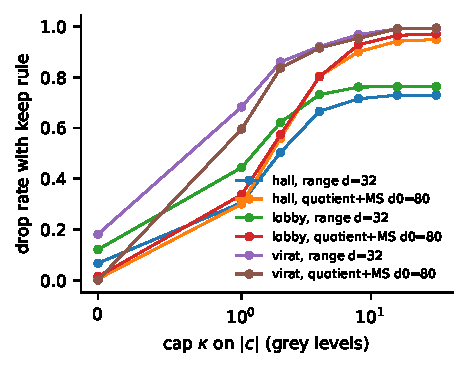
\includegraphics[width=0.55\linewidth]{figures/shift_cost}
\caption{Drop rate against the cap $\kappa$ on the brightness shift (Table~\ref{tab:shift}). Above $\kappa \approx 16$ the cap costs almost nothing.}
\label{fig:shift}
\end{figure}
